\section{知识链接}
\subsection{平面图形分析}
要准确地绘制复杂的图样,我们需要了解一定的平面图形分析知识,才能够更准确快捷的绘出图样。图样上的图形是平面图形,需要用尺寸确定组成图样的若干封闭线框的形状(定形尺寸)和相互位置(定位尺寸)。这些形(图形)和数(尺寸)的关系对于设计和加工人员来说是十分重要的。因此,我们必须要弄清楚图形与尺寸之的关系。

\subsubsection{平面图形的尺寸分析}
尺寸分析包括尺寸基准、定形尺寸和定位尺寸的分析。

\begin{figure}[htbp]
\centering
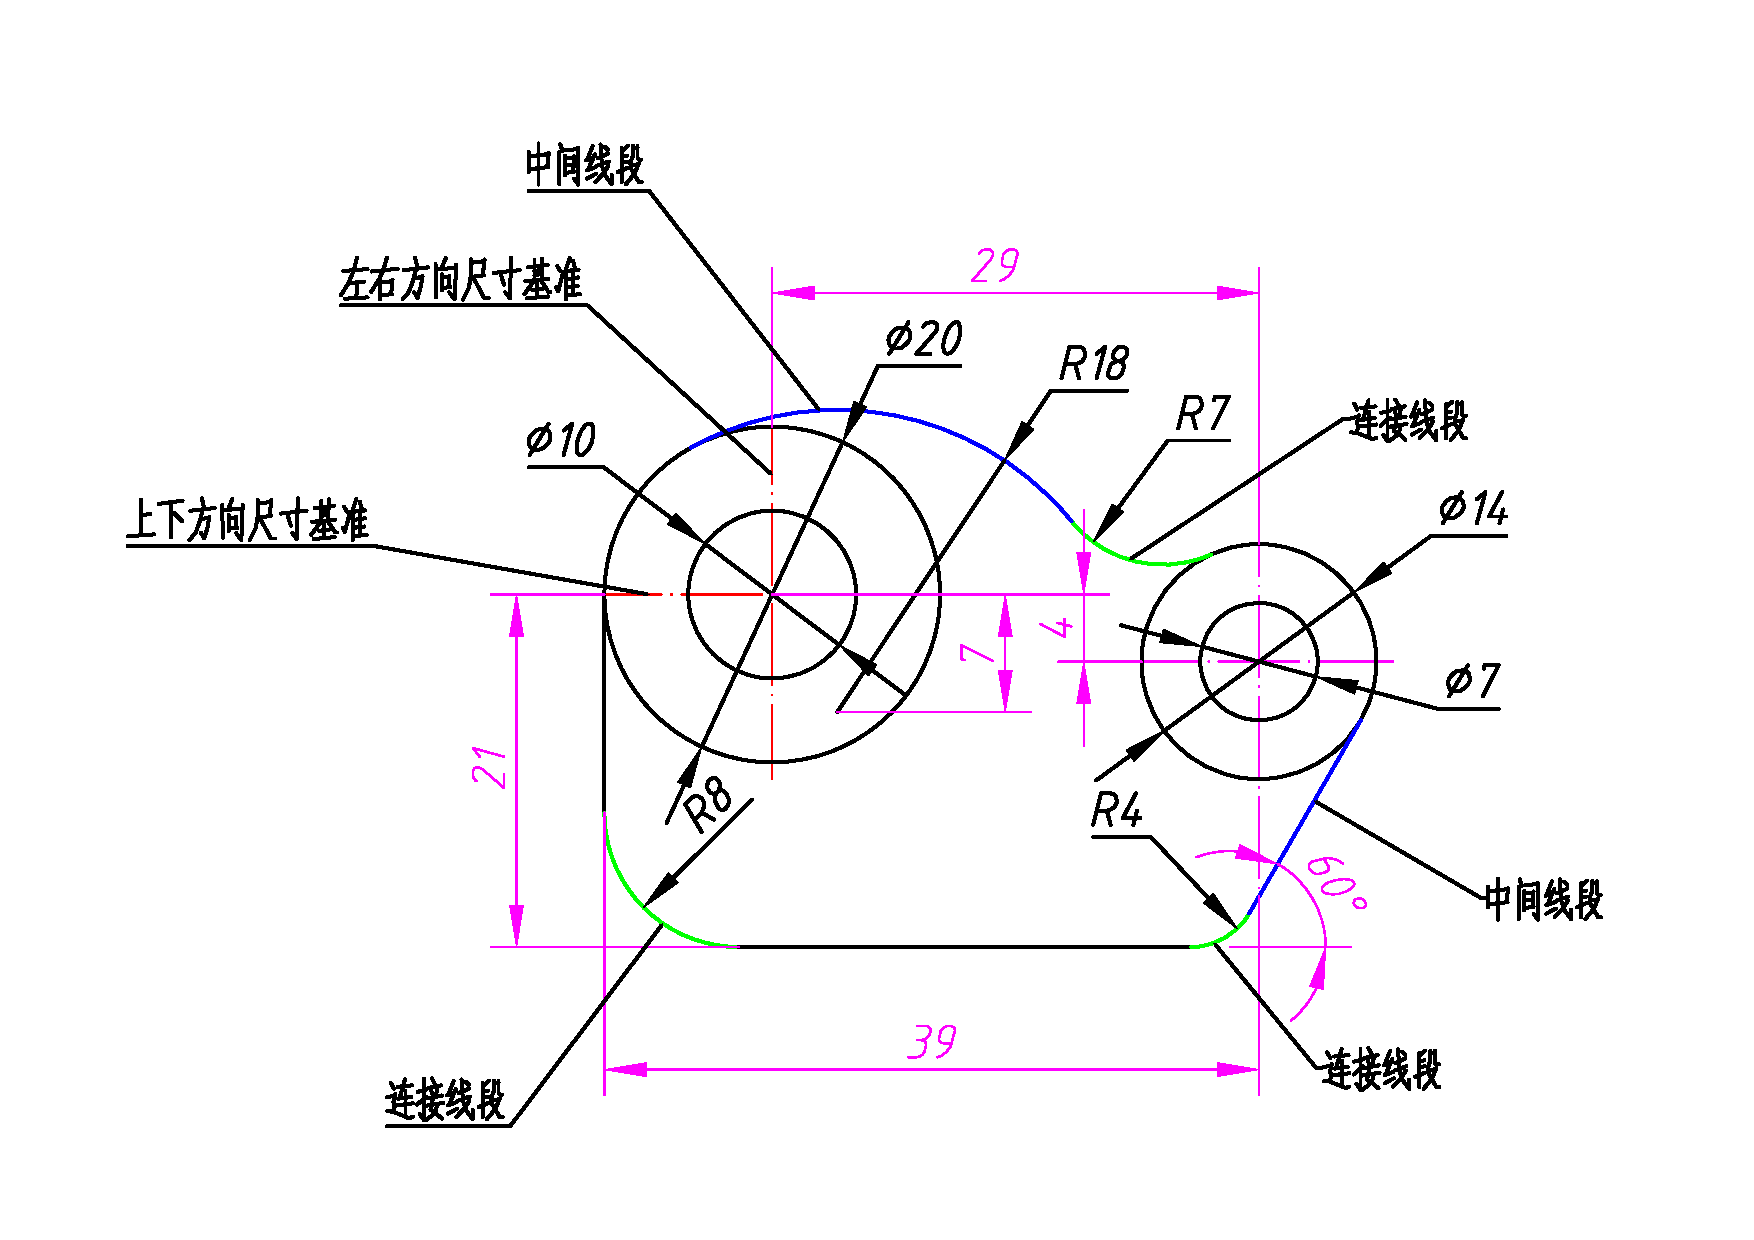
\includegraphics[scale=0.35]{biaozu.pdf}
\caption{平面图形的尺寸和线段分析} \label{fig:biaozu}
\end{figure}

\begin{enumerate}
\item 尺寸基准

尺寸基准是标注尺寸的起点。一般应有两个方向的尺寸基准。通常情况下,平面图形主要采用图形的对称中心线,较大圆的中心线或主要轮廓线作为尺寸基准线。如图\ref{fig:biaozu}所示,则是采用$\phi 20$圆的中心线作为上下方向和左右方向的尺寸基准。

\item 定形尺寸

定形尺寸是确定平面图形中各线段形状大小的尺寸,如直线的长度、圆和圆弧的直径或半径、角度的大小等。图\ref{fig:biaozu6}所标出的$\phi 10$、$\phi 20$、 $\phi 14$、 $R8$、$R18$、$R7$等尺寸均为图\ref{fig:biaozu}的定形尺寸。

\begin{figure}[htbp]
\centering
\begin{floatrow}
\ffigbox{\caption{定形尺寸}\label{fig:biaozu6}}{
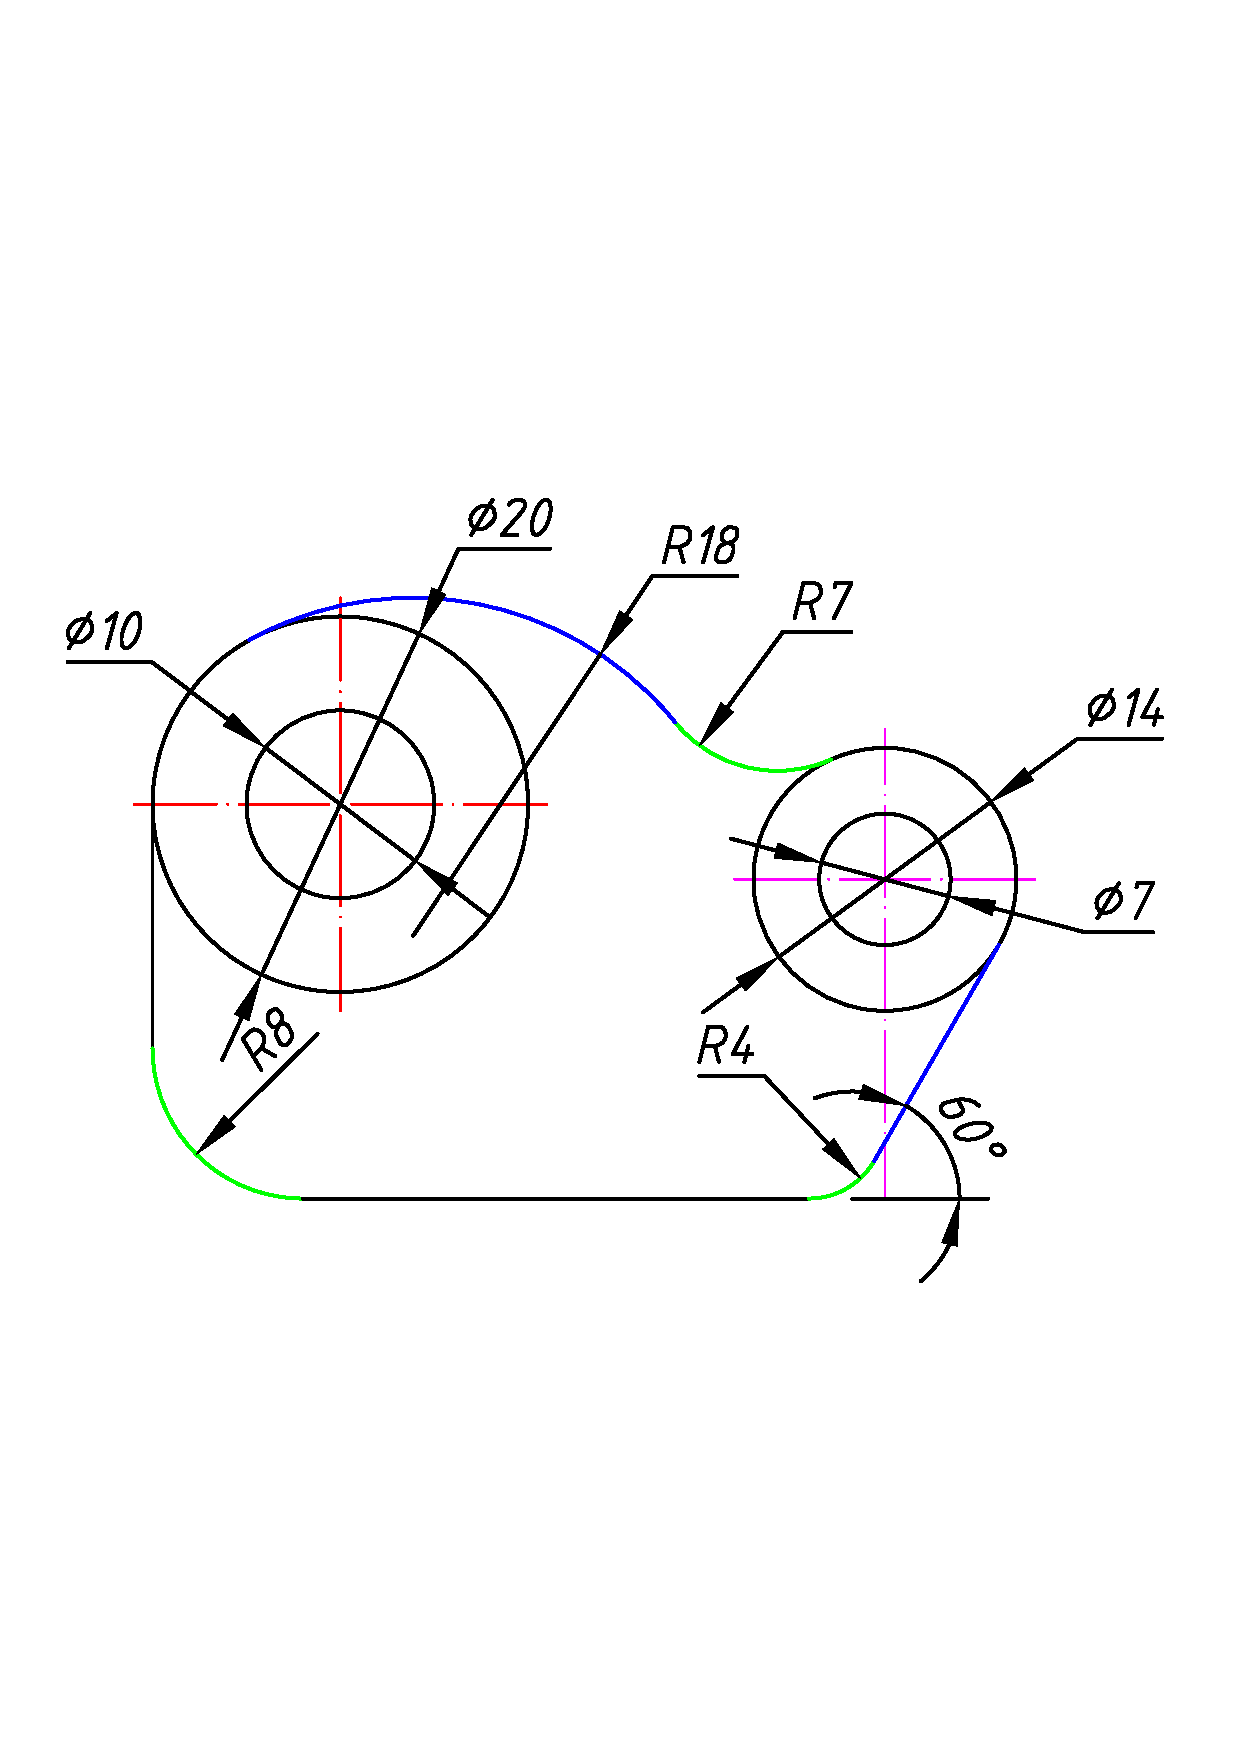
\includegraphics[scale=0.25]{biaozu6.pdf}
}
\ffigbox{\caption{定位尺寸}\label{fig:biaozu5}}{
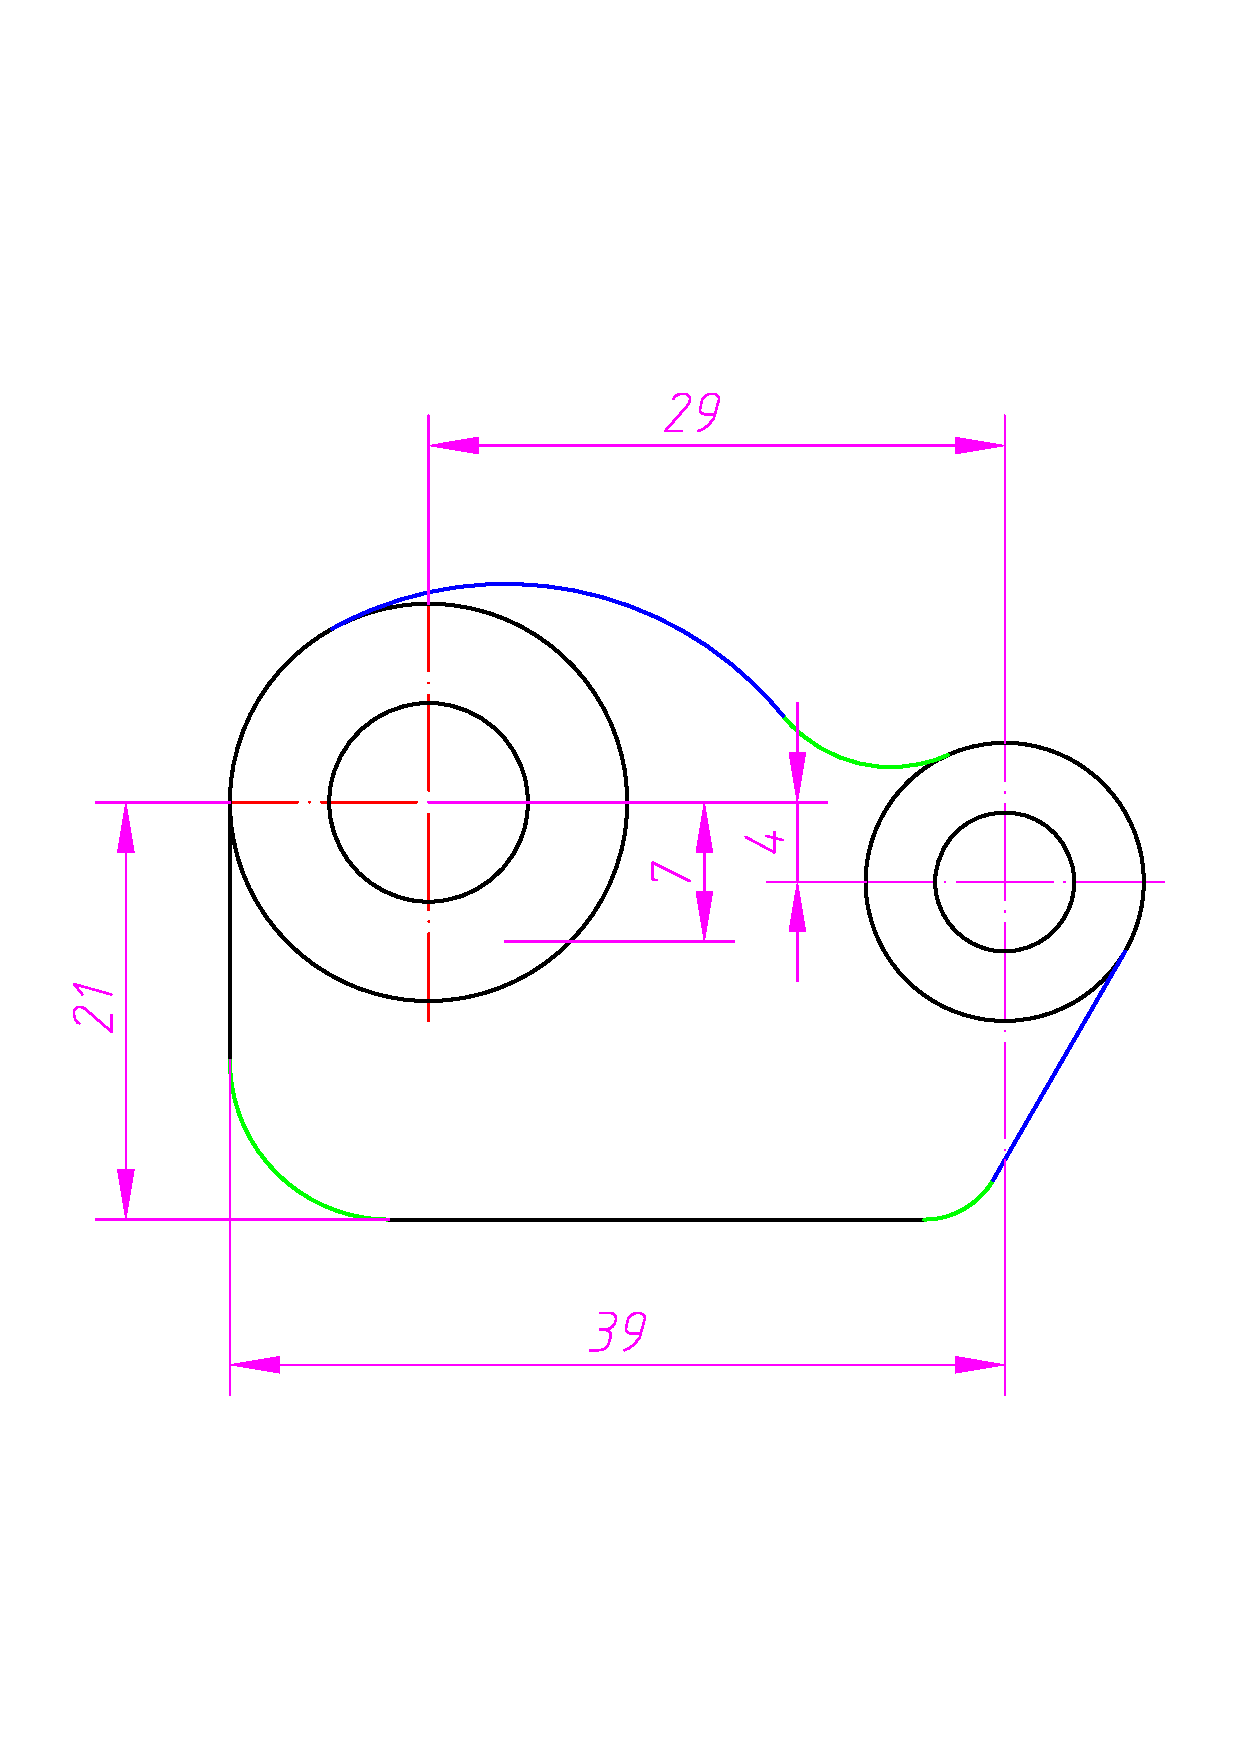
\includegraphics[scale=0.2]{biaozu5.pdf}
}
\end{floatrow}
\end{figure}

\item 定位尺寸

定位尺寸是确定平面图形中各线段之间相对位置的尺寸,如图\ref{fig:biaozu5}所标出的尺寸均为图\ref{fig:biaozu}的定位尺寸,其中4和29用于确定$\phi 14$圆的圆心位置。

\end{enumerate}
\subsubsection{平面图形中线段性质的分析}
平面图形中各线段(直线或圆弧)的定位尺寸的数量将直接影响绘图先后顺序,因此可将线段分为以下三类。

\begin{enumerate}
\item 已知线段

已知线段是有足够的定形尺寸,不需要利用与其它线段的连接关系即可直接画出的直线或圆弧。图\ref{fig:biaozu2}所示的即为图\ref{fig:biaozu}的已知线段。

\item 中间线段

中间线段是缺少一个定位尺寸,需要通过与它相邻某一边的图线的连接关系,才能够作出的直线或圆弧。图\ref{fig:biaozu3}在图\ref{fig:biaozu2}的基础上绘制出所有的中间线段。
\item 连接线段

连接线段是缺少两定位尺寸,需要通过与它相邻两边图形的相切关系,才能够作出的直线或圆弧。图\ref{fig:biaozu4}在图\ref{fig:biaozu3}的基础上进一步添加所有的连接线段。
\end{enumerate}

\begin{figure}[htbp]
\centering
\subfloat[已知线段]{\label{fig:biaozu2}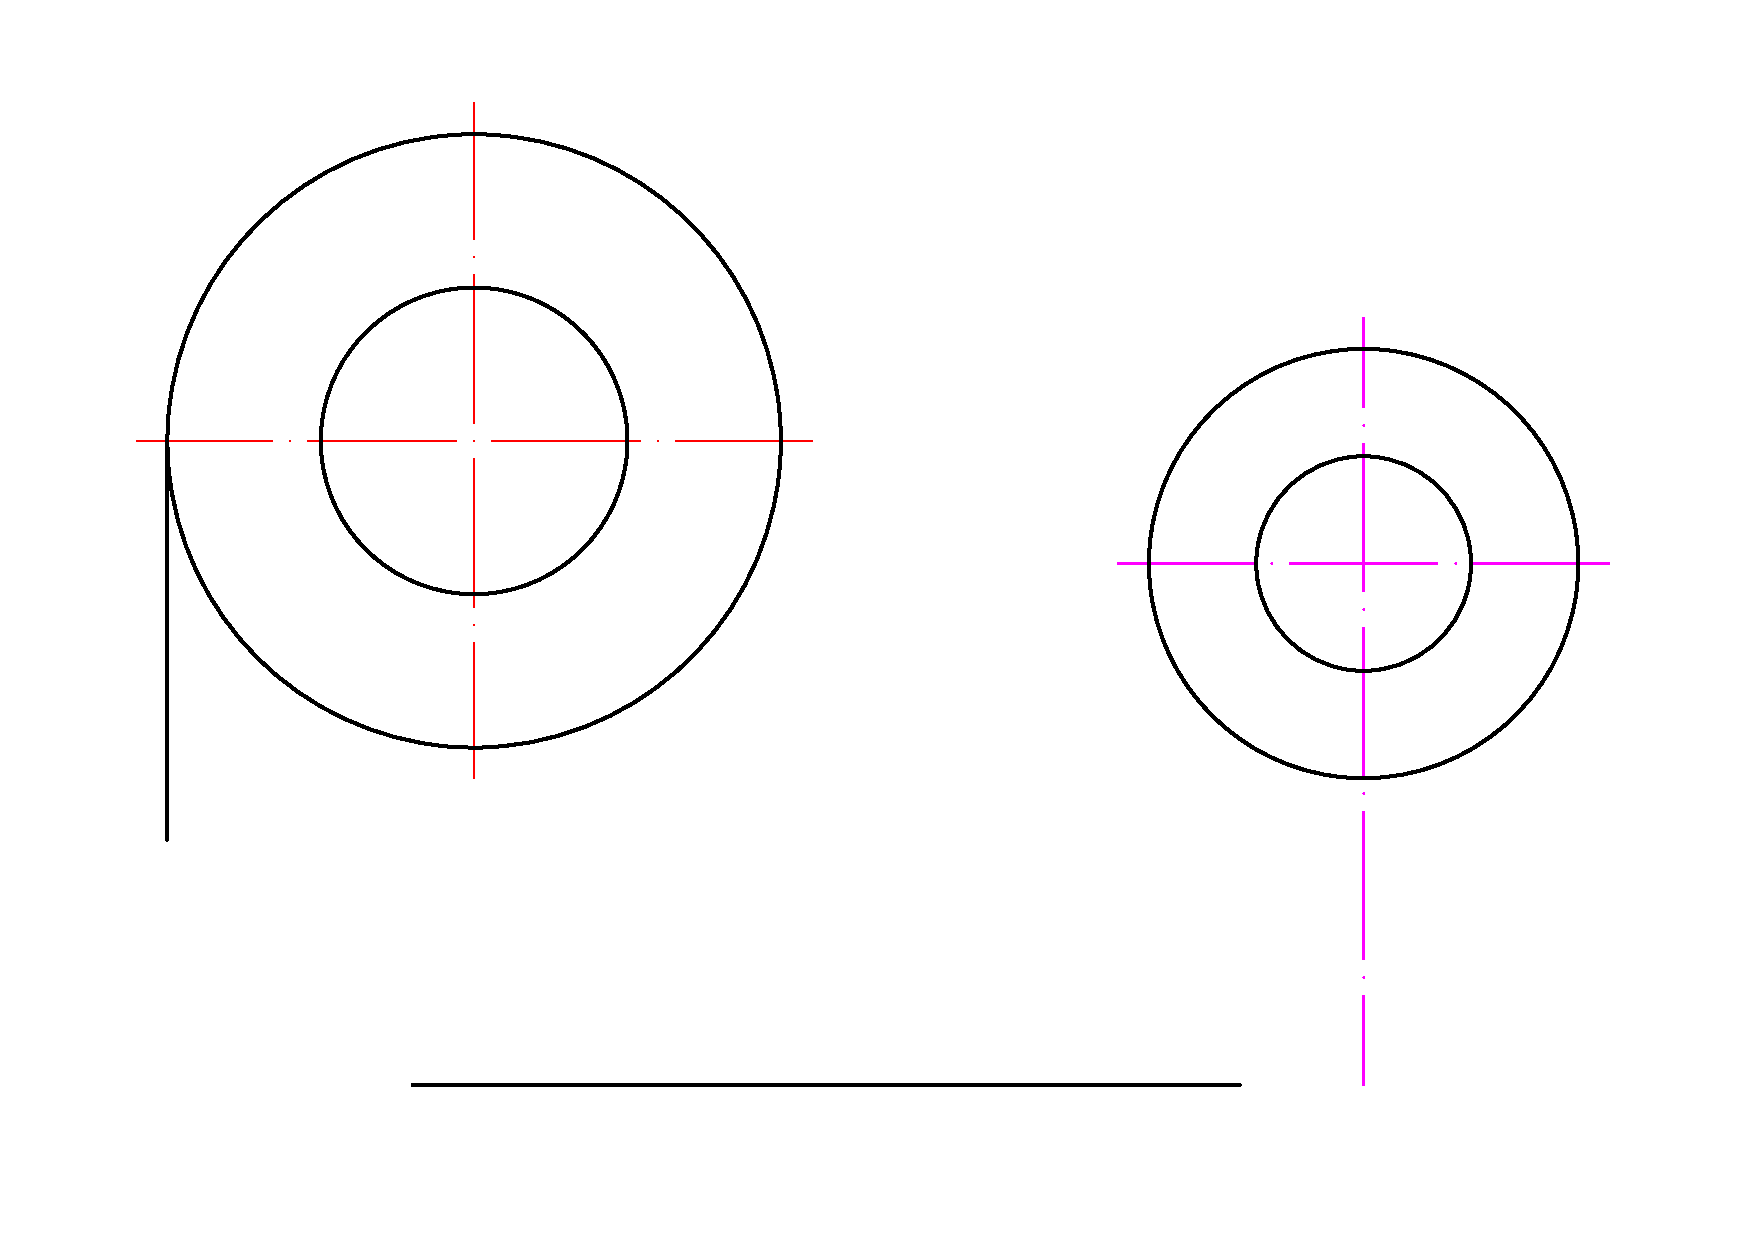
\includegraphics[scale=0.15]{biaozu2.pdf}}\hspace{20pt}
\subfloat[中间线段]{\label{fig:biaozu3}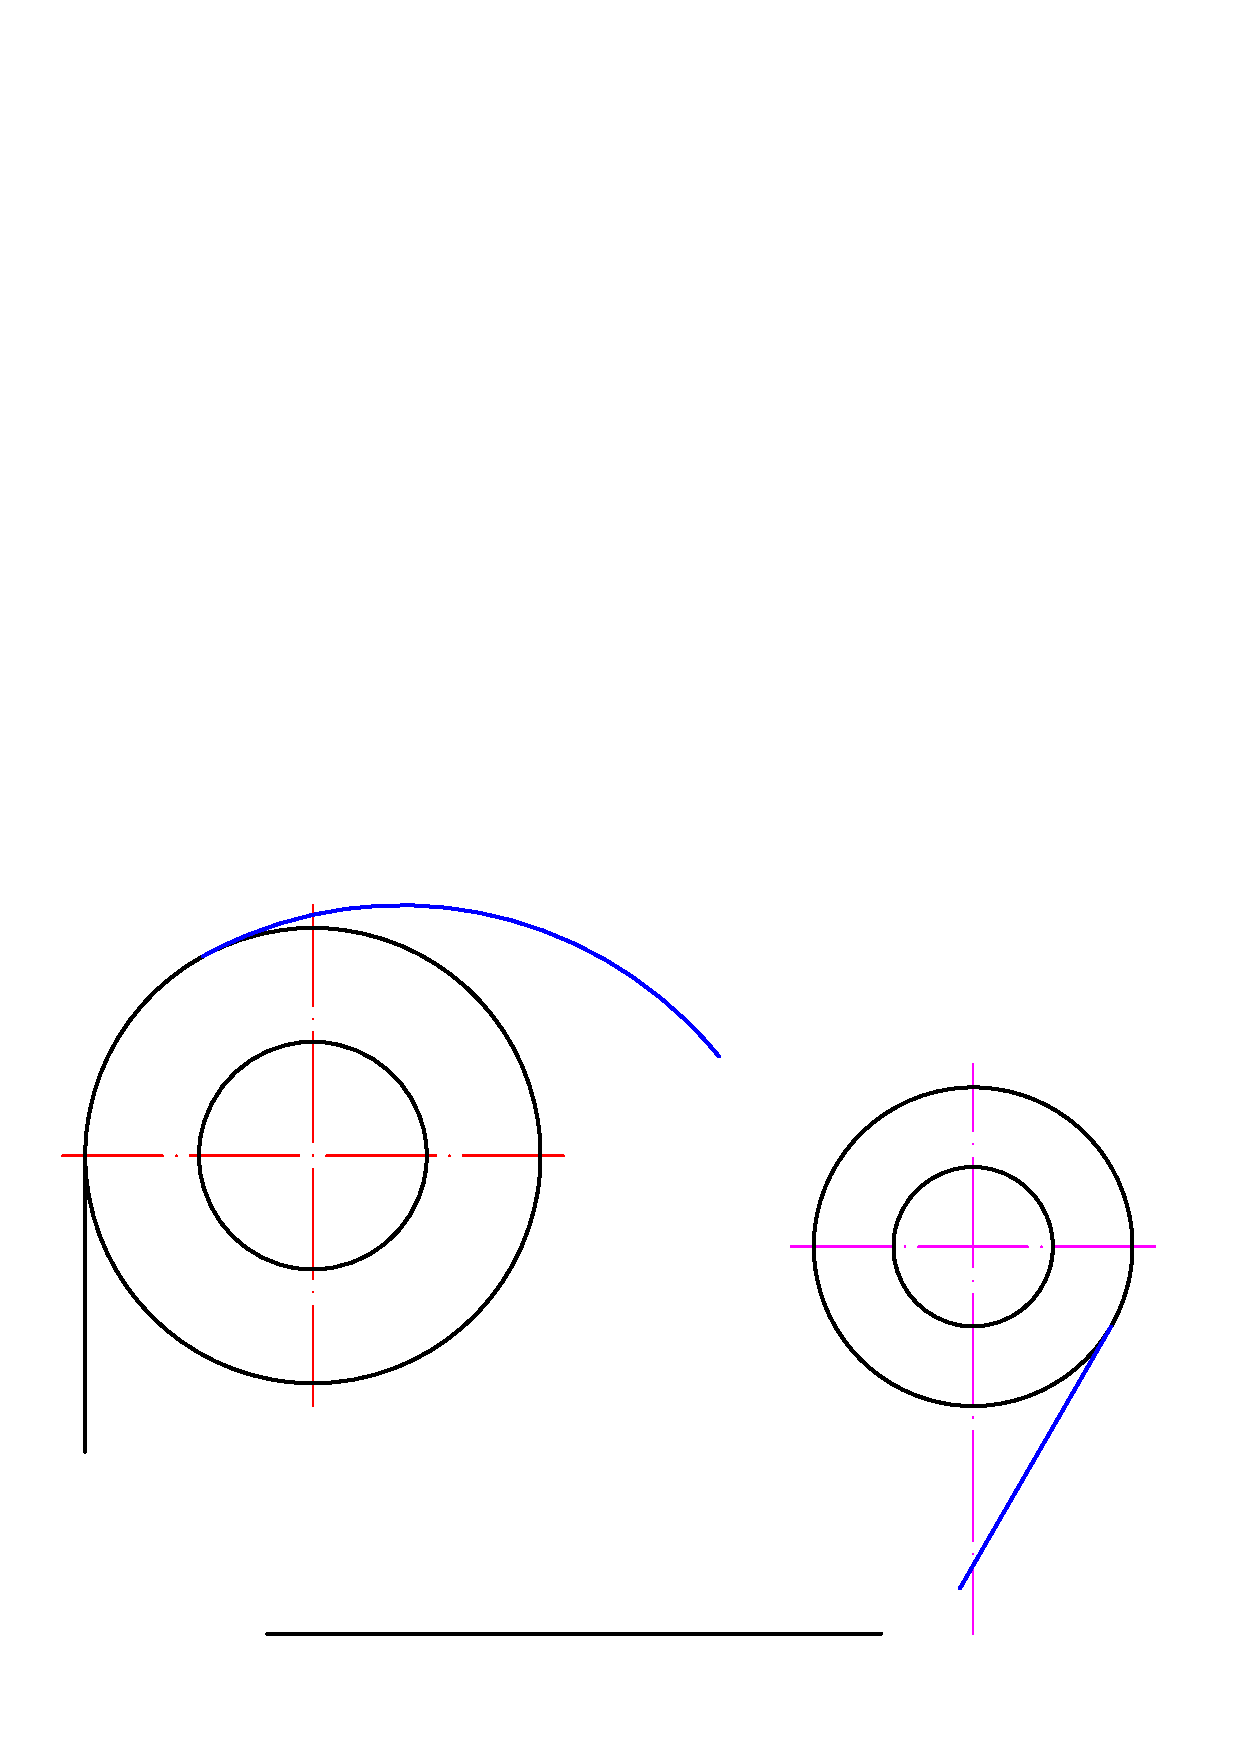
\includegraphics[scale=0.2]{biaozu3.pdf}}\hspace{20pt}
\subfloat[连接线段]{\label{fig:biaozu4}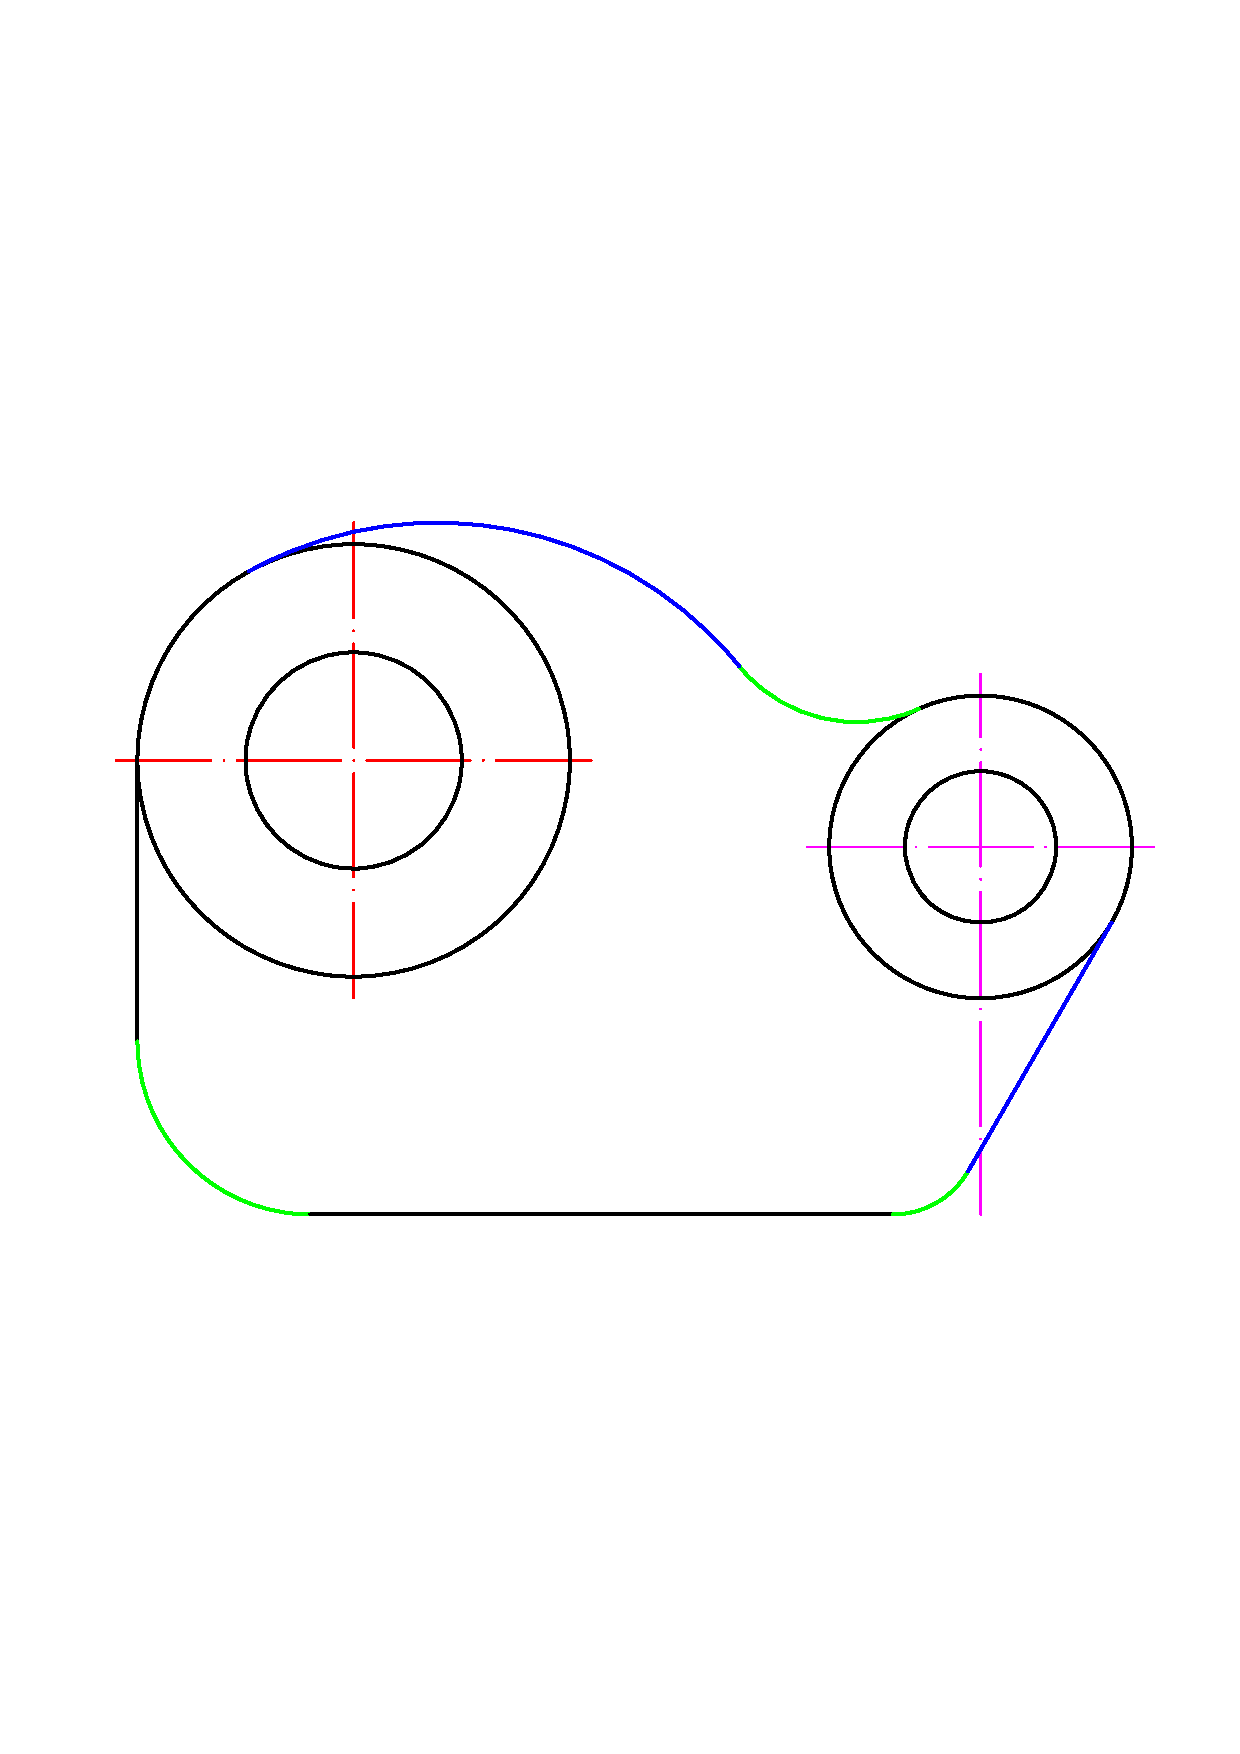
\includegraphics[scale=0.2]{biaozu4.pdf}}
\caption{平面图形中的线段分析}
\end{figure}

\subsection{图样绘制方法和步骤}
\subsubsection{CAD绘图流程}
\begin{enumerate}
\item 设置图层。根据绘图样所需要的线型创建图层并设置其颜色、线型、线宽等参数。
\item 画图框及标题栏。
\item 确定绘图比例,布置图形,使图形在图纸上的位置和大小适中,各图形间应留有适当空隙及标注尺寸的位置。
\item 绘制图样。先画图形的基准线、对称线、中心线及有关定位尺寸线,再根据定型尺寸画主要轮廓线,然后由大到小,由整体到局部,画出其他所有图线。
\item 标注尺寸(将在后续任务中详细讲解)。
\end{enumerate}
\subsubsection{手工绘图流程}
\begin{enumerate}
\item 画图前的准备工作
    \begin{enumerate}
    \item 阅读必要的参考资料,对所画图形的内容与要求进行了解。
    \item 准备好必要的制图工具,将铅笔与圆规内的铅削好。
    \item 固定图纸
    \end{enumerate}
\item 画底稿
\begin{enumerate}
\item 画图框及标题栏(前两个任务省略了此过程)。
\item 确定绘图比例,布置图形,使图形在图纸上的位置和大小适中,各图形间应留有适当空隙及标注尺寸的位置。
\item 绘制图样。先画图形的基准线、对称线、中心线及有关定位尺寸线,再根据定型尺寸画主要轮廓线,然后由大到小,由整体到局部,画出其他所有图线。
\item 标注尺寸(将在后续任务中详细讲解)。
\end{enumerate}
\item 加深图线。按照先细后粗,先曲线后直线,先图形后尺寸,先图线后符号、文字的顺序,从上到下,从左到右进行。

\end{enumerate}

\endinput